\documentclass[12pt,english]{article}
\usepackage[T1]{fontenc}
\usepackage{amsmath}
\usepackage{babel}
\usepackage{graphicx}
\graphicspath{{../images/}}

\author{
    Meisel, Carlos \\
  \and
  Juarez, Albert\\
  \and
    Quintero, Osvaldo\\
}
\title{Task 5 - Compressor Airfoil CFD}
\begin{document}
  \maketitle

\section{Overview}
This report contains the results of the CFD analysis performed on the compressor airfoil our team has chosen from Task 3.


\section{Flow Conditions}
As defined in the \textit{T.L. User's Manual}, the flow through a cascade is defined by two parameters:
\begin{itemize}
\item The inlet flow Mach number $M_{in}$
\item inlet flow angle $\alpha_{in}$
\end{itemize}

We have two non-dimensional parameters that define the flow through the cascade:

\begin{equation}
\label{eq:non-dim rho}
\rho_{in} = 1
\end{equation}

\begin{equation}
\label{eq:non-dim v}
V_{in} = 1
\end{equation}

Where, $\rho_{in}$ is the static density at the inlet and $V_{in}$ is the velocity at the inlet.  
From here we can calculate the Mach number at the inlet:

\begin{equation}
\label{eq:inlet mach}
M_{in} = \frac{V_{in}}{c_{in}}
\end{equation}

Since $V_{in}$ is a non-dimensional parameter, we need to non-dimensionalize the speed of sound $c_{in}$. 
We can do this by taking a look at how $V_{in}$ is defined:

\begin{equation}
\label{eq:def inlet velocity}
V_{in} = \frac{157.5}{157.5}
\end{equation}

Applying the same logic to the speed of sound we get:

\begin{equation}
\label{eq:def inlet speed of sound}
c_{in} = \frac{\sqrt{\gamma R T}}{157.5}
\end{equation}

Where $\gamma$ is the ratio of specific heats, $R$ is the gas constant and $T$ is the temperature.
Since this all takes place in the compressor, the working fluid is air, meaning that $\gamma = 1.4$
and $R = 287.058 \frac{J}{kgK}$.

Resulting in our Mach number to be:

\begin{equation}
\label{eq:mach}
M_{in} = 0.462823
\end{equation}

We are then able to calculate the static pressure at the inlet:

\begin{equation}
\label{eq:inlet pressure}
p_{in} = \frac{1}{\gamma M_{in}^2}
\end{equation}

Readers may recall the standard isentropic relations for pressure and density from AERO 201:

\begin{equation}
\label{eq:isentropic pressure}
p_{0} = p \left( 1 + \frac{\gamma-1}{2} M^{2} \right)^{\frac{\gamma}{\gamma - 1}}
\end{equation}

\begin{equation}
\label{eq:isentropic density}
\rho_{0} = \rho \left( 1 + \frac{\gamma-1}{2} M^{2} \right)^{\frac{1}{\gamma - 1}}
\end{equation}

We can makew use of these relations to calculate the total pressure and density at the inlet:

\begin{equation}
\label{eq:total pressure}
p_{0_{in}} = p_{in} \left( 1 + \frac{\gamma-1}{2} M_{in}^{2} \right)^{\frac{\gamma}{\gamma - 1}}
\end{equation}

\begin{equation}
\label{eq:total density}
\rho_{0_{in}} = \rho_{in} \left( 1 + \frac{\gamma-1}{2} M_{in}^{2} \right)^{\frac{1}{\gamma - 1}}
\end{equation}

We calculated our total parameters to be:

\begin{equation}
\label{eq:total pressure}
p_{0_{in}} = 2.87924668
\end{equation}

\begin{equation}
\label{eq:total density}
\rho_{0_{in}} = 0.9004399
\end{equation}

We induced a flow angle of $\alpha_{in} = 44.6$ degrees. 
Alowing for us to calculate the:

\begin{equation}
\label{eq:FLUX}
\verb|FLUX| = V_{in} \cos{\alpha_{in}}
\end{equation}

\begin{equation}
\label{eq:VTAN}
\verb|VTAN| = V_{in} \sin{\alpha_{in}}
\end{equation}

Resulting in:

\begin{center}
  $\verb|FLUX| = 0.712026045991$ \\
  $\verb|VTAN| = 0.702153052995$ \\
  $\verb|UINIT| = 0.712026045991$ \\
  $\verb|VINIT| = 0.702153052995$ \\
\end{center}

\section{Computational Fluid Dynamics Figures}

\begin{figure}[h]
  \centering
  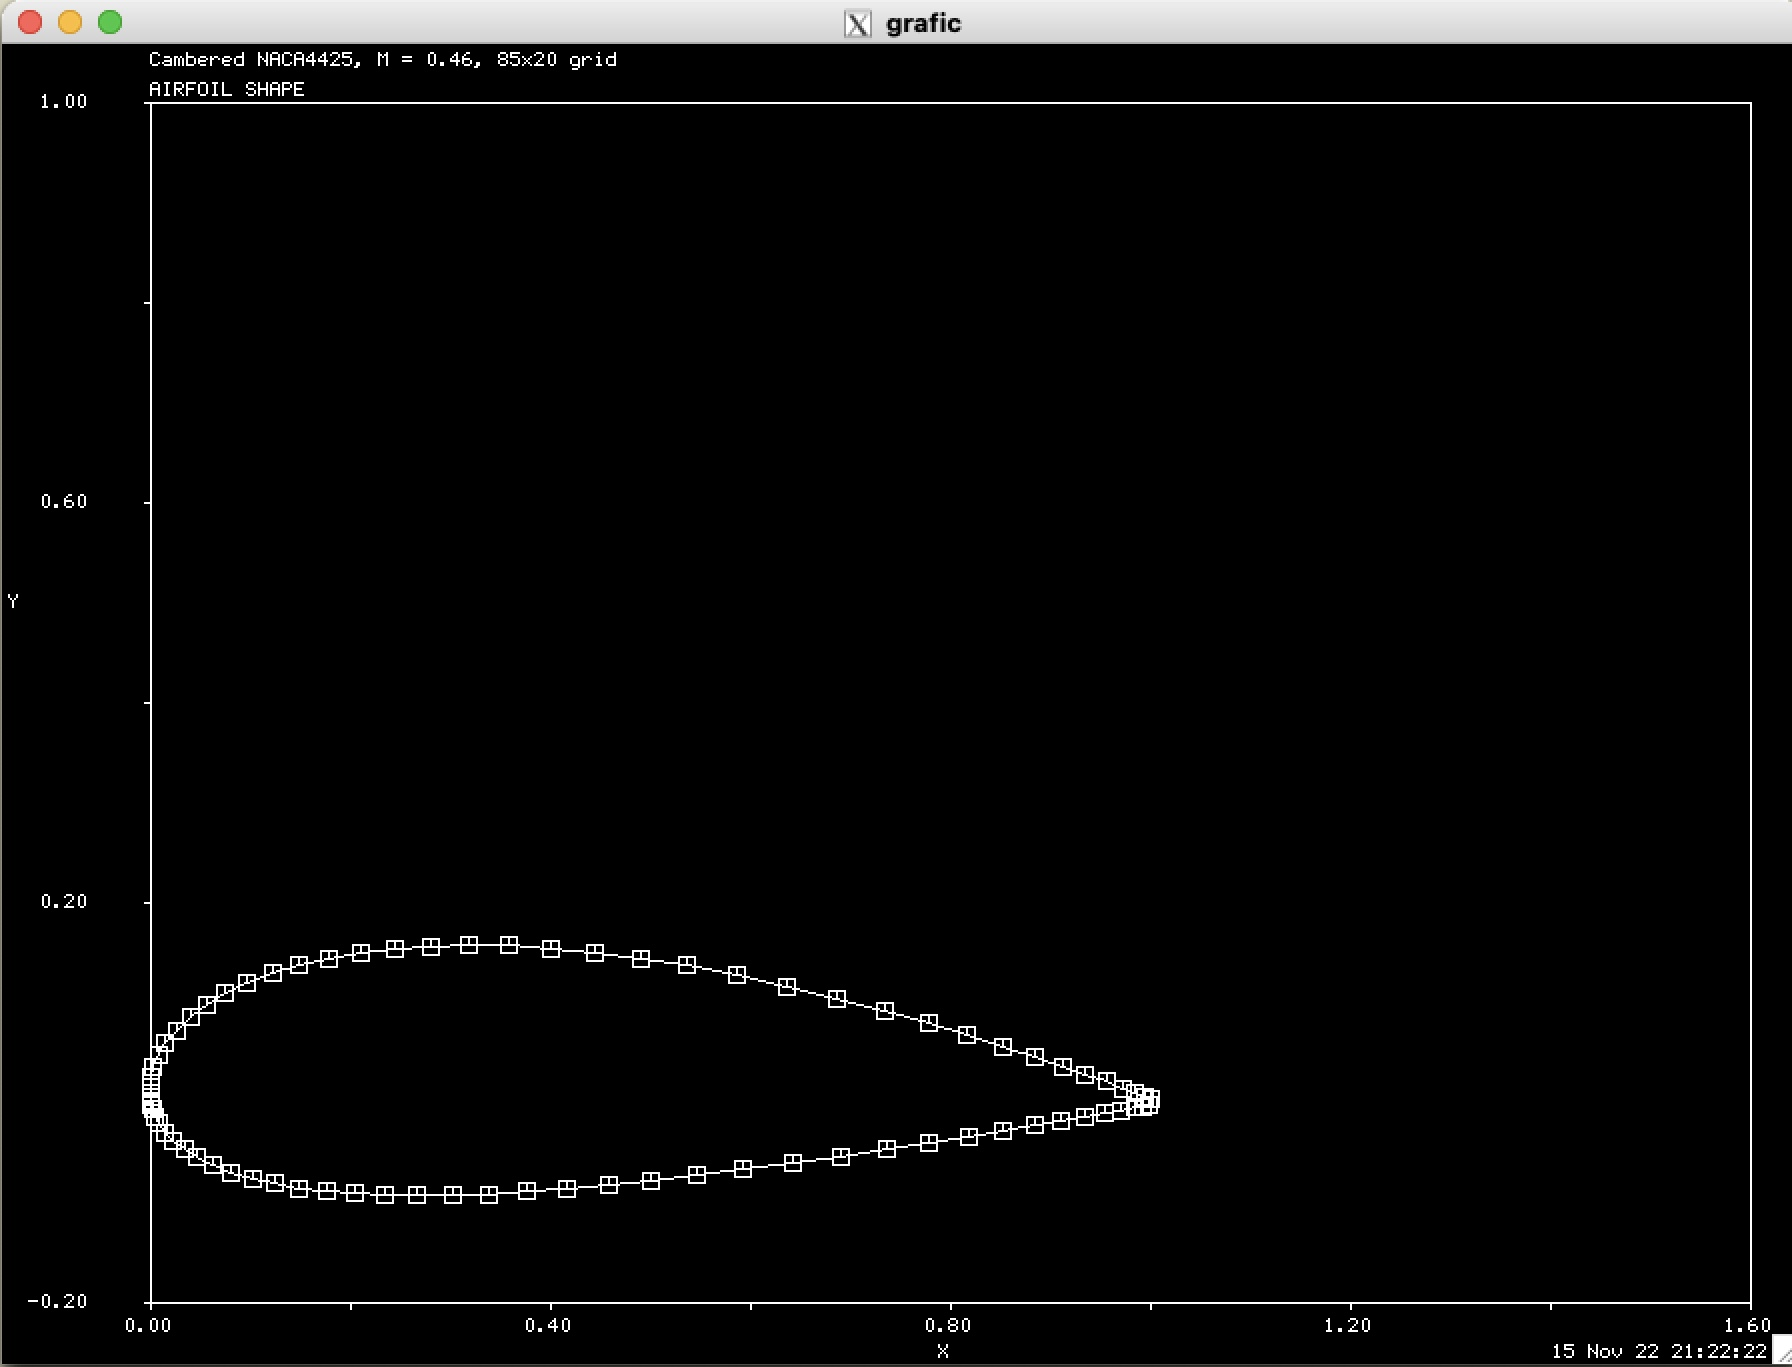
\includegraphics[width=1.0\textwidth]{/airfoil1.jpeg}
  \caption{Plot of the airfoil shape (recomputed)}
  \label{fig:Airfoil1}
\end{figure}

\begin{figure}[h]
  \centering
  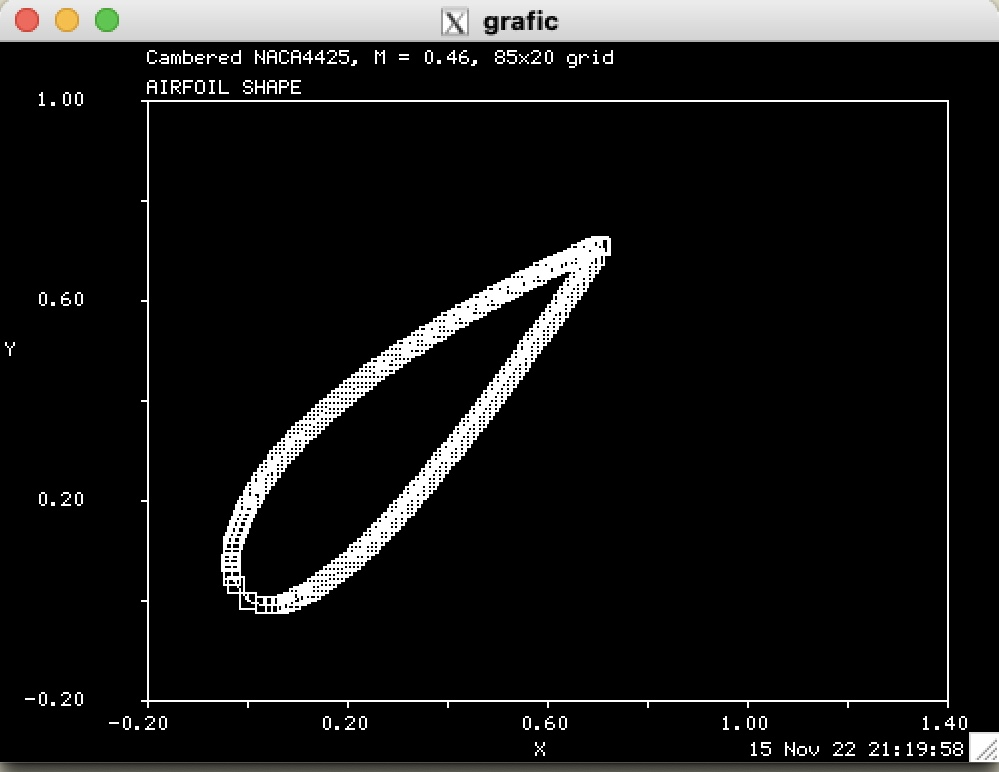
\includegraphics[width=1.0\textwidth]{/airfoil2.jpeg}
  \caption{Plot of the airfoil shape (cascade definition)}
  \label{fig:Airfoil2}

\end{figure}

\begin{figure}[h]
  \centering
  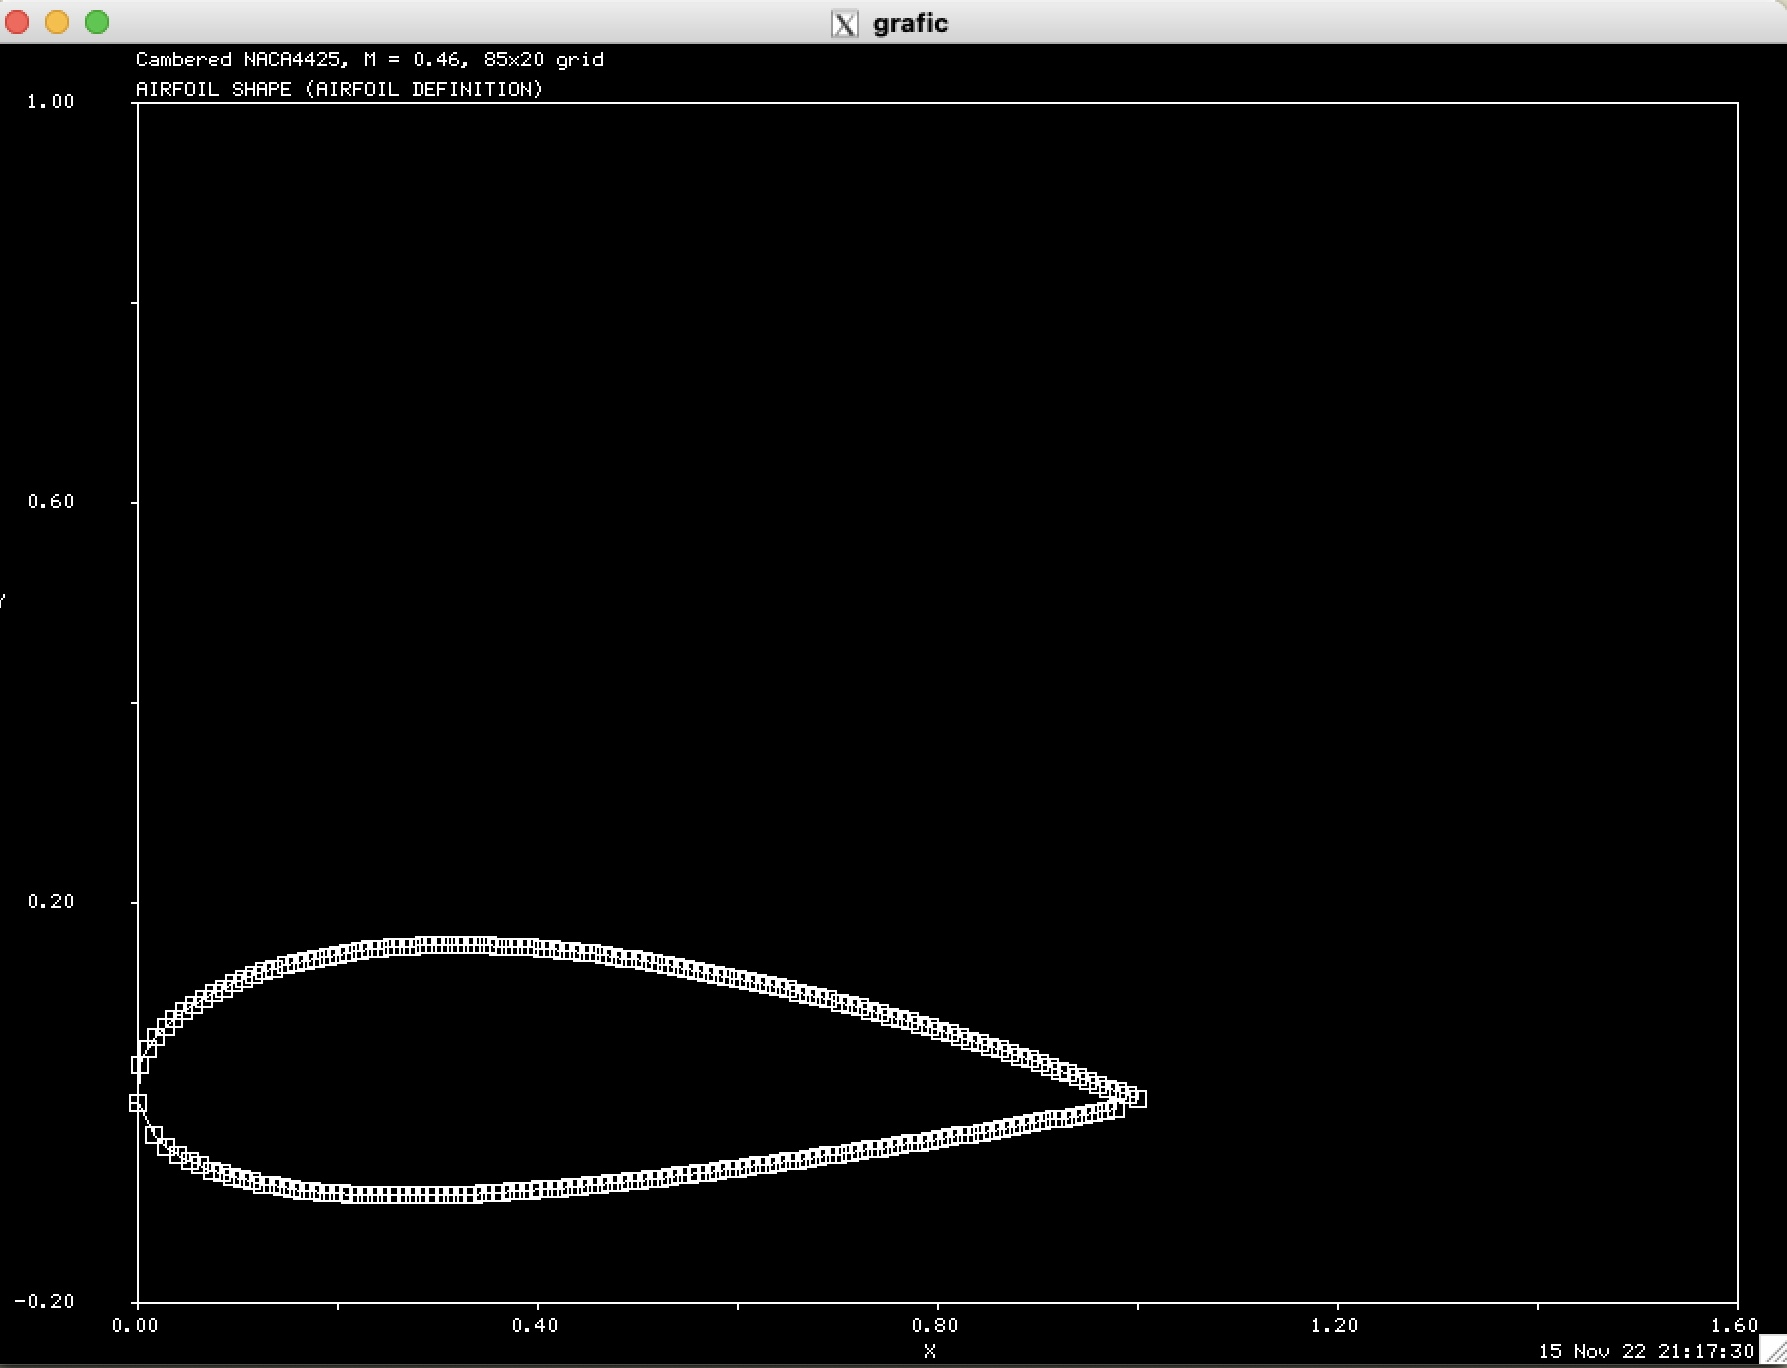
\includegraphics[width=1.0\textwidth]{/airfoil3.jpeg}
  \caption{Plot of the airfoil shape (airfoil definition)}
  \label{fig:Airfoil3}
\end{figure}


\begin{figure}[h]
  \centering
  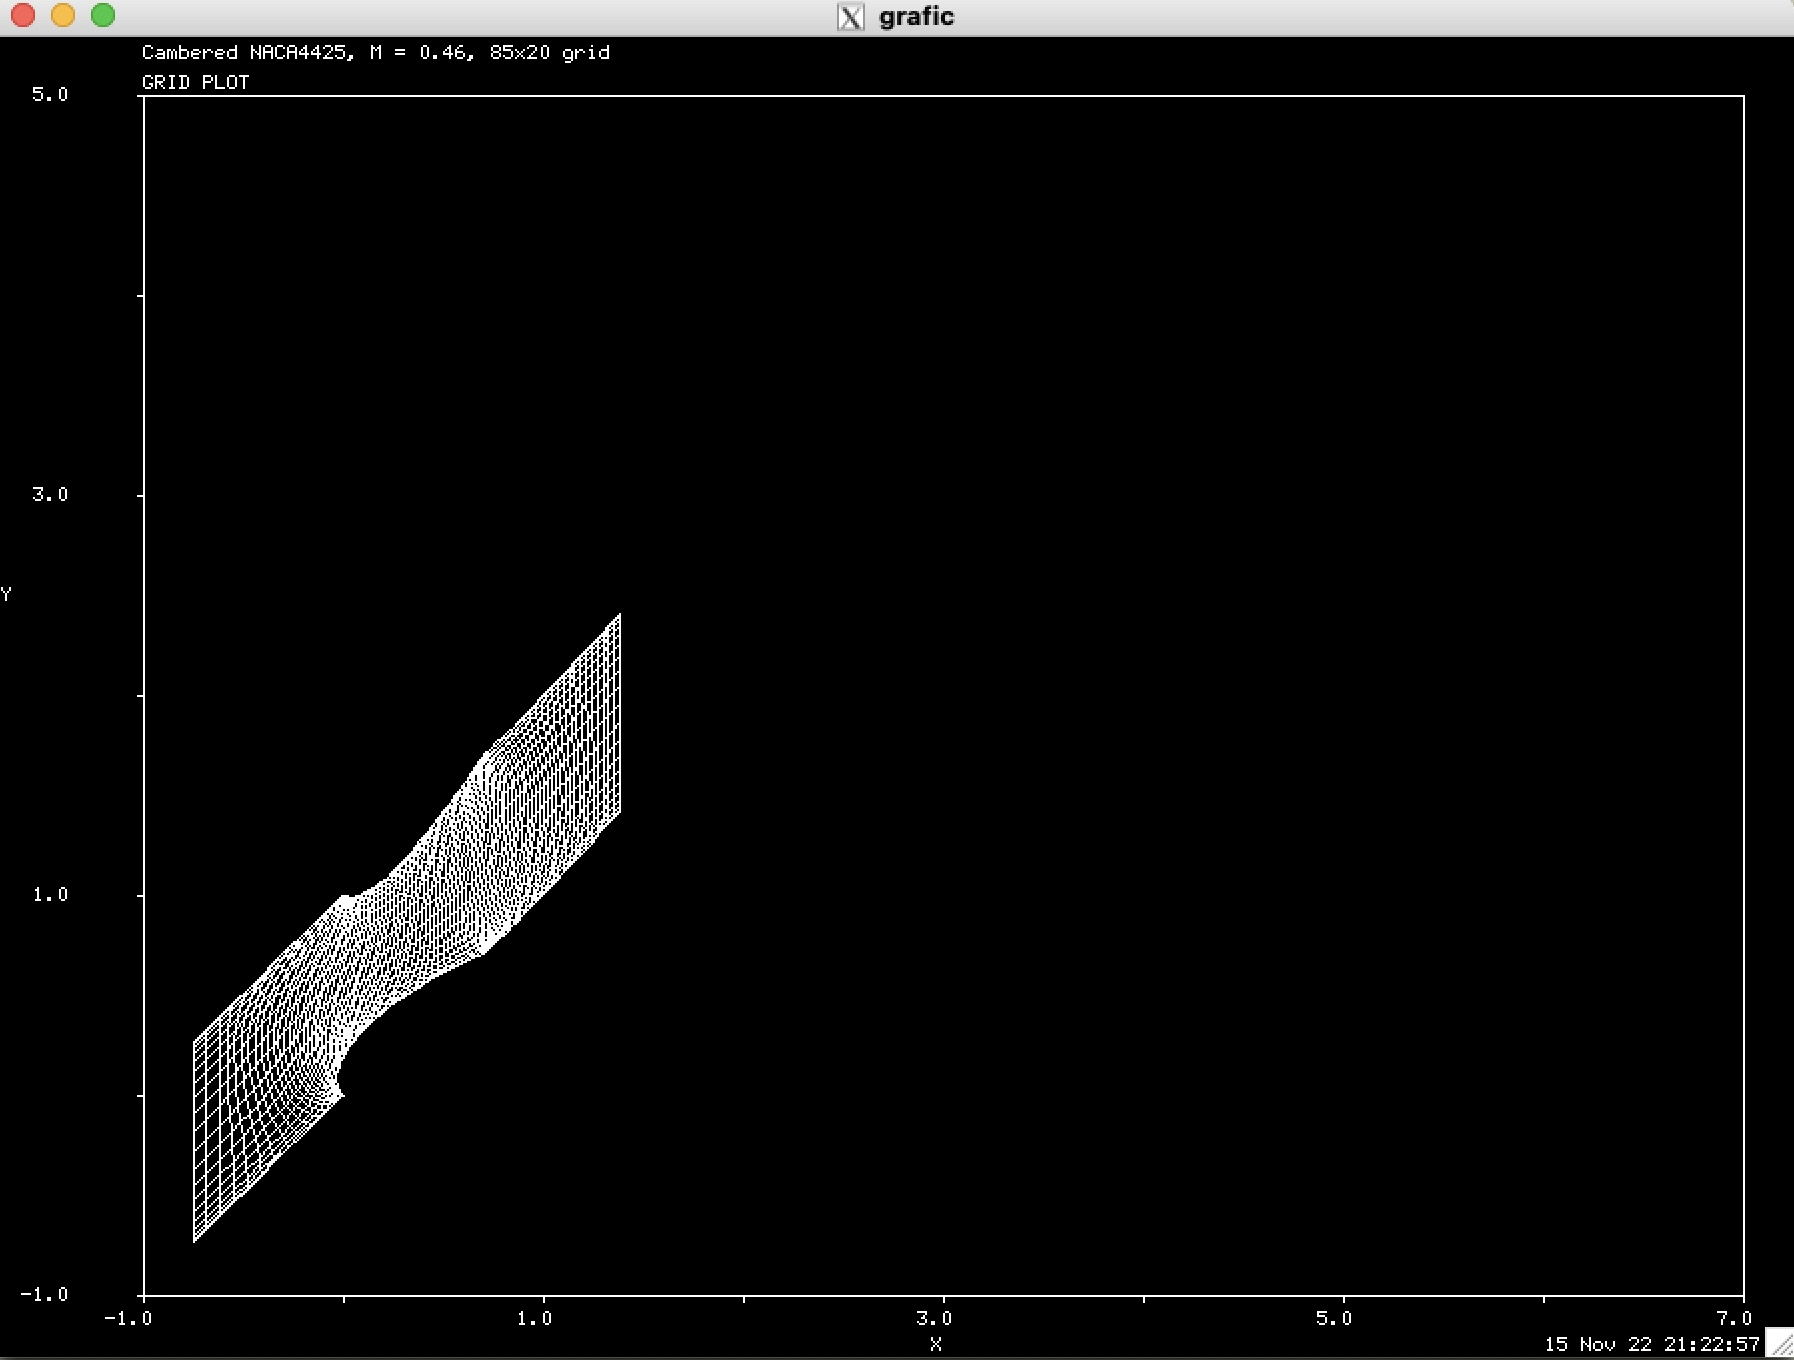
\includegraphics[width=1.0\textwidth]{/compgrid.jpeg}
  \caption{Plot of the Computational Grid used}
  \label{fig:CompGrid}
\end{figure}

\begin{figure}[h]
  \centering
  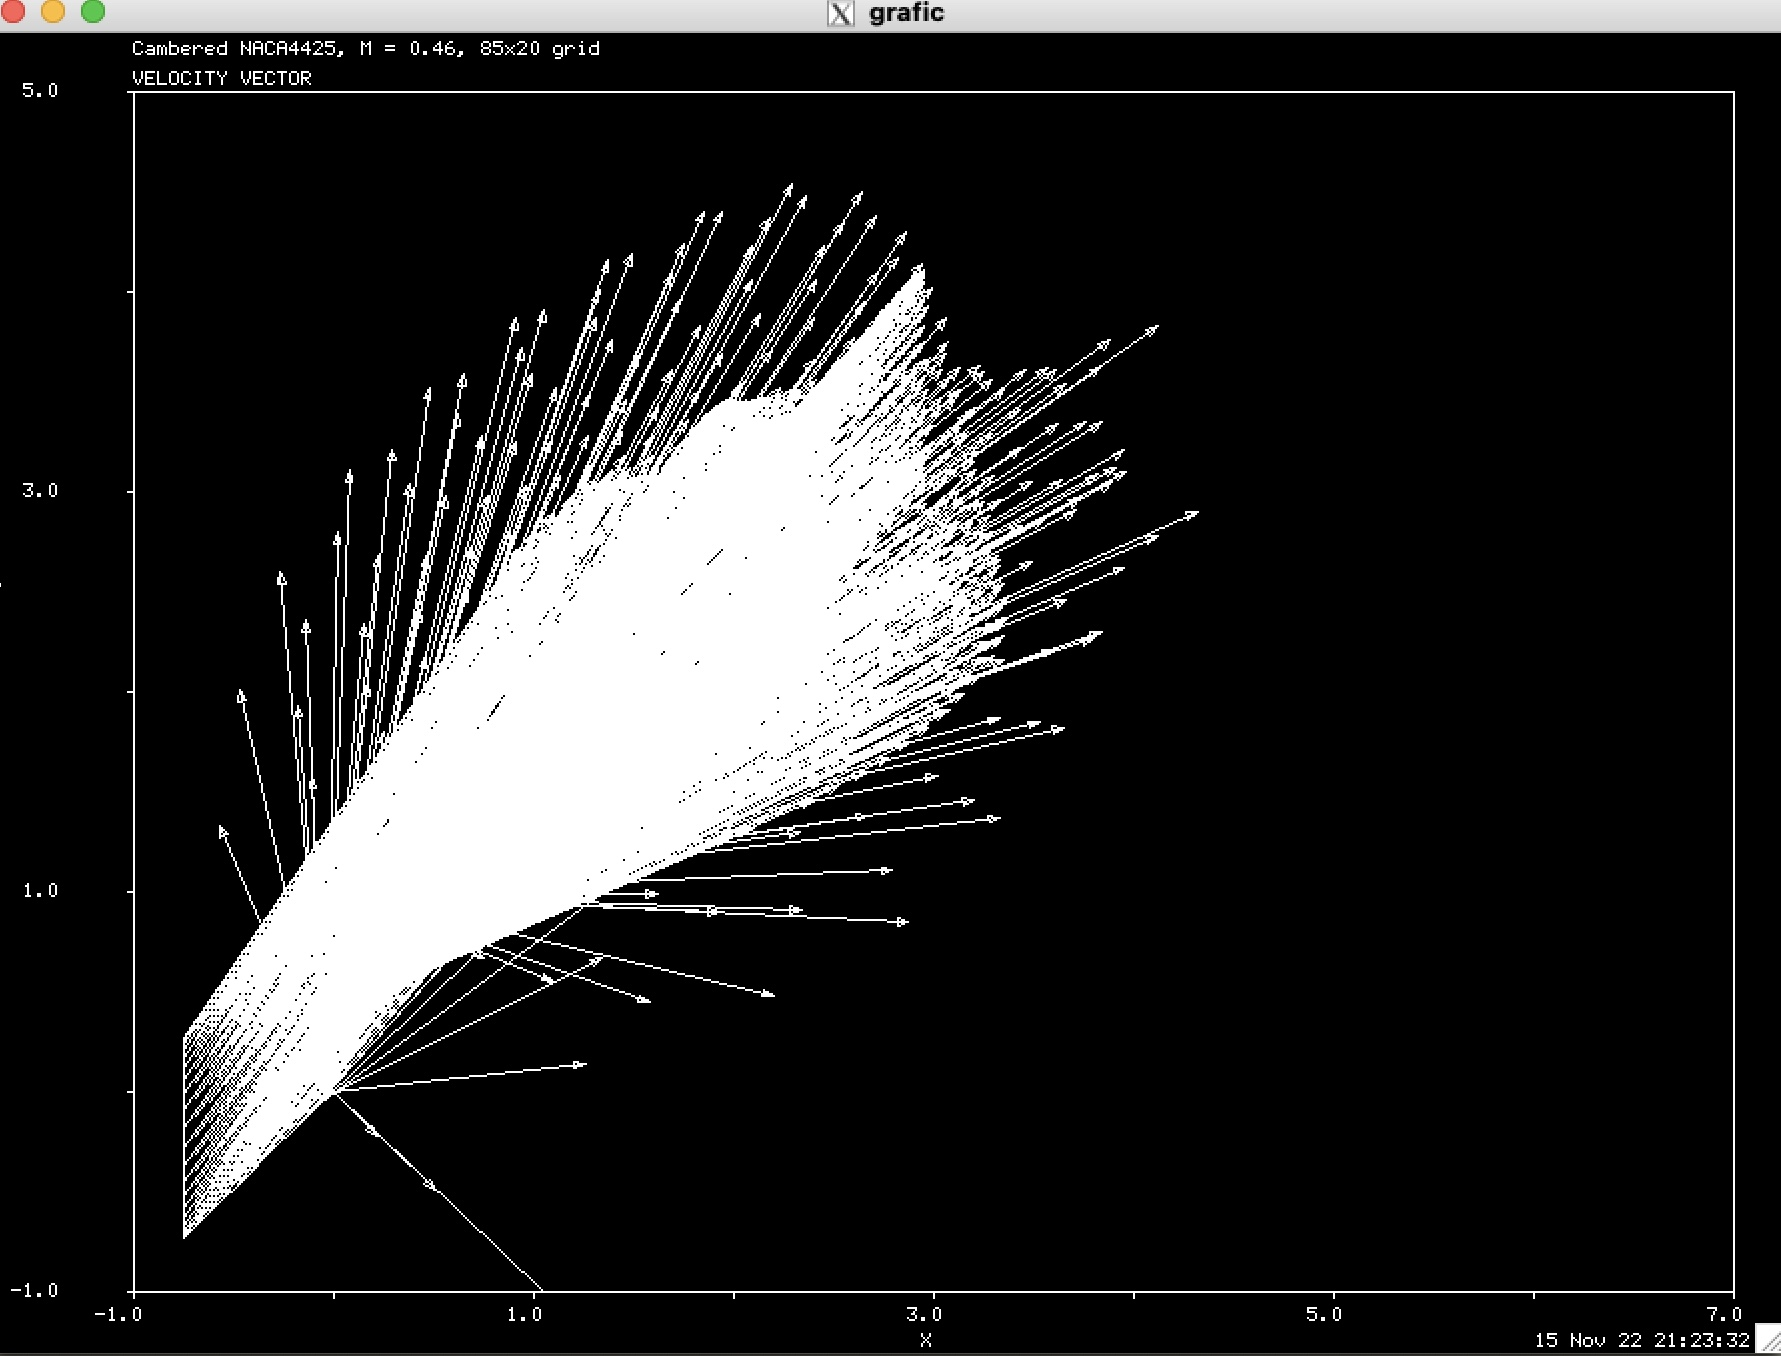
\includegraphics[width=1.0\textwidth]{/velocity.jpeg}
  \caption{Plot the the Velocity Vectors}
  \label{fig:Vel Vectors}
\end{figure}

\begin{figure}[h]
  \centering
  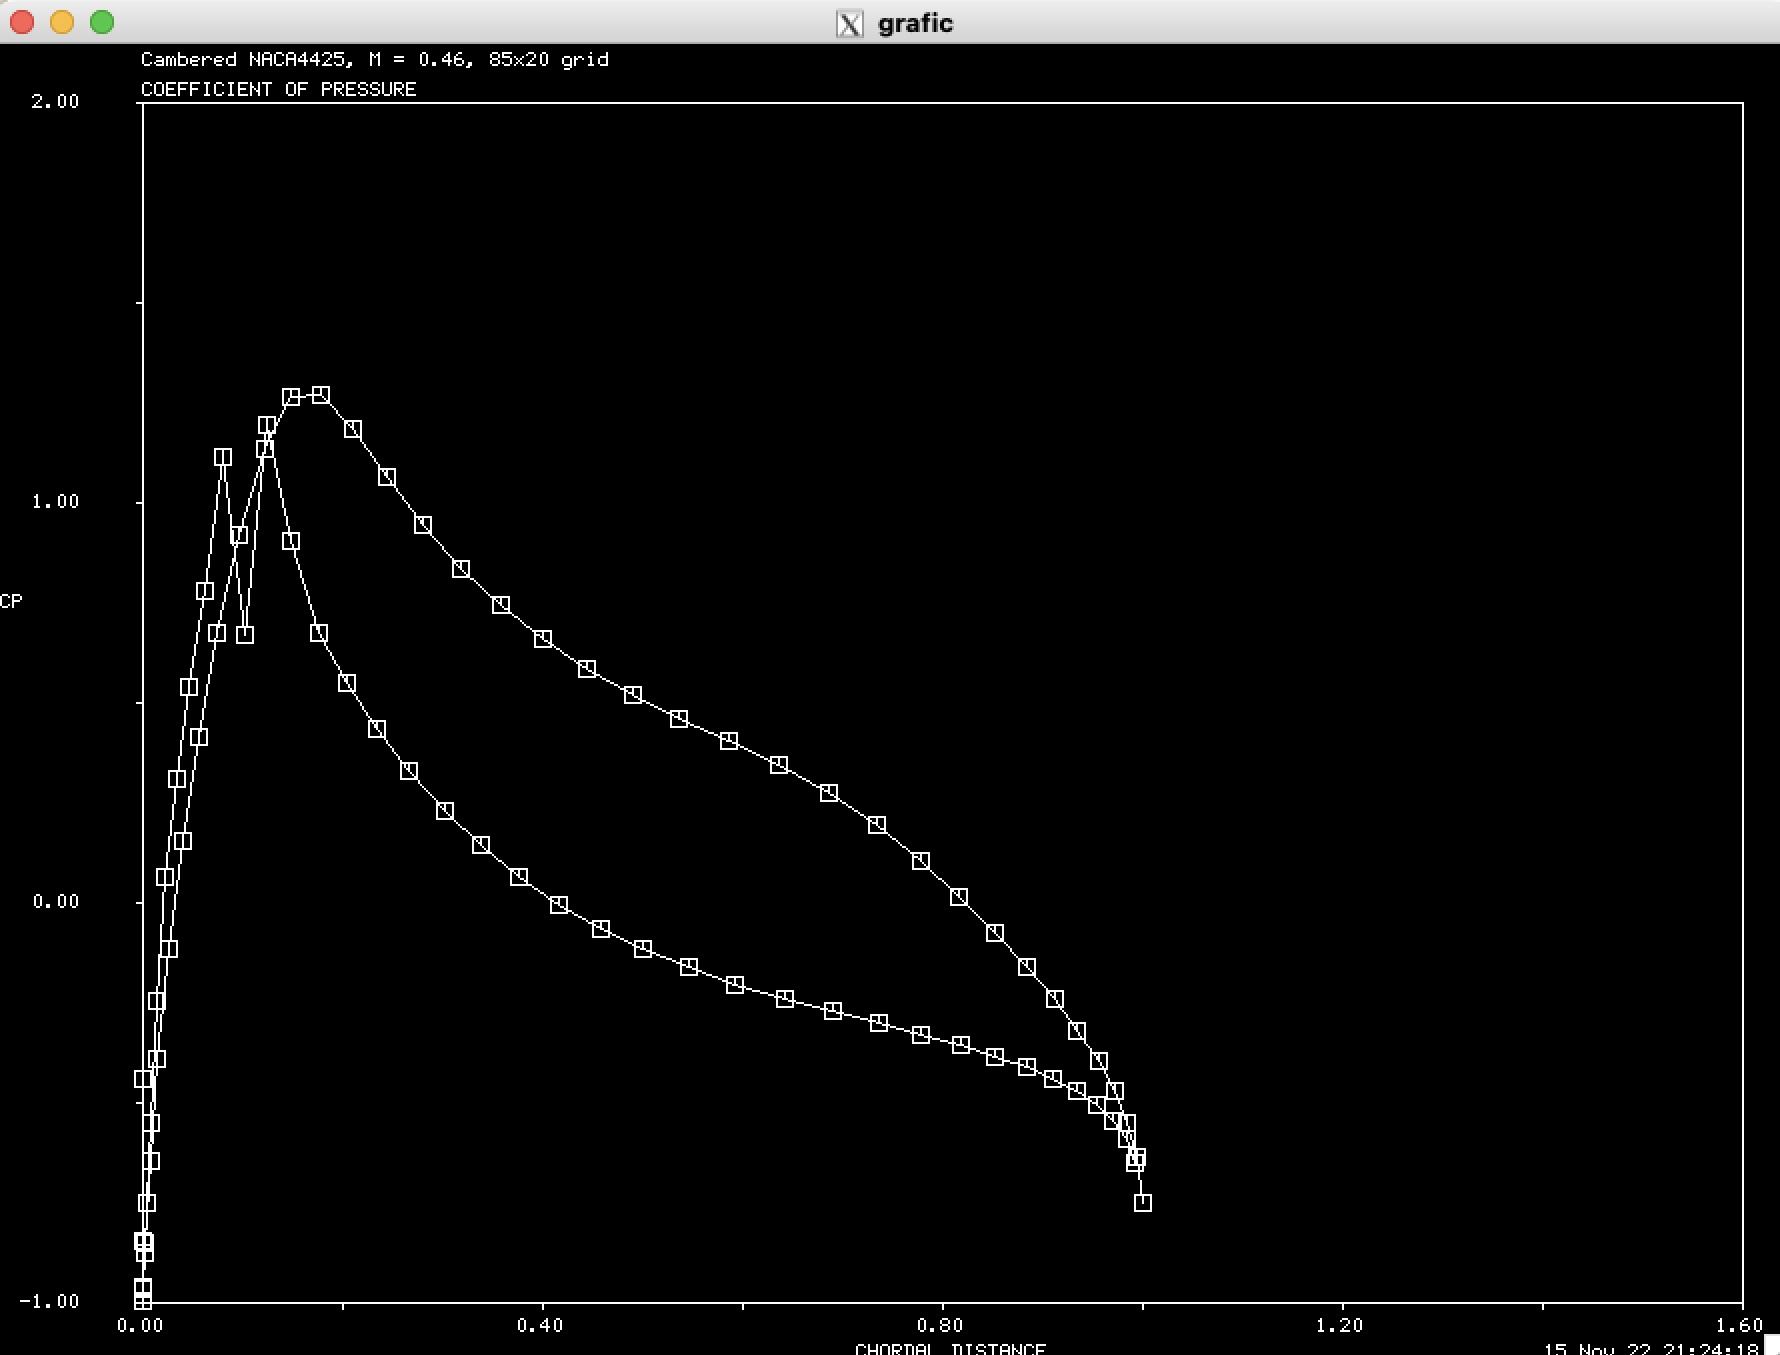
\includegraphics[width=1.0\textwidth]{/Pressure.jpeg}
  \caption{Plot of the Surface Pressure Coefficient}
  \label{fig:Pressure Coef}
\end{figure}

\begin{figure}[h]
  \centering
  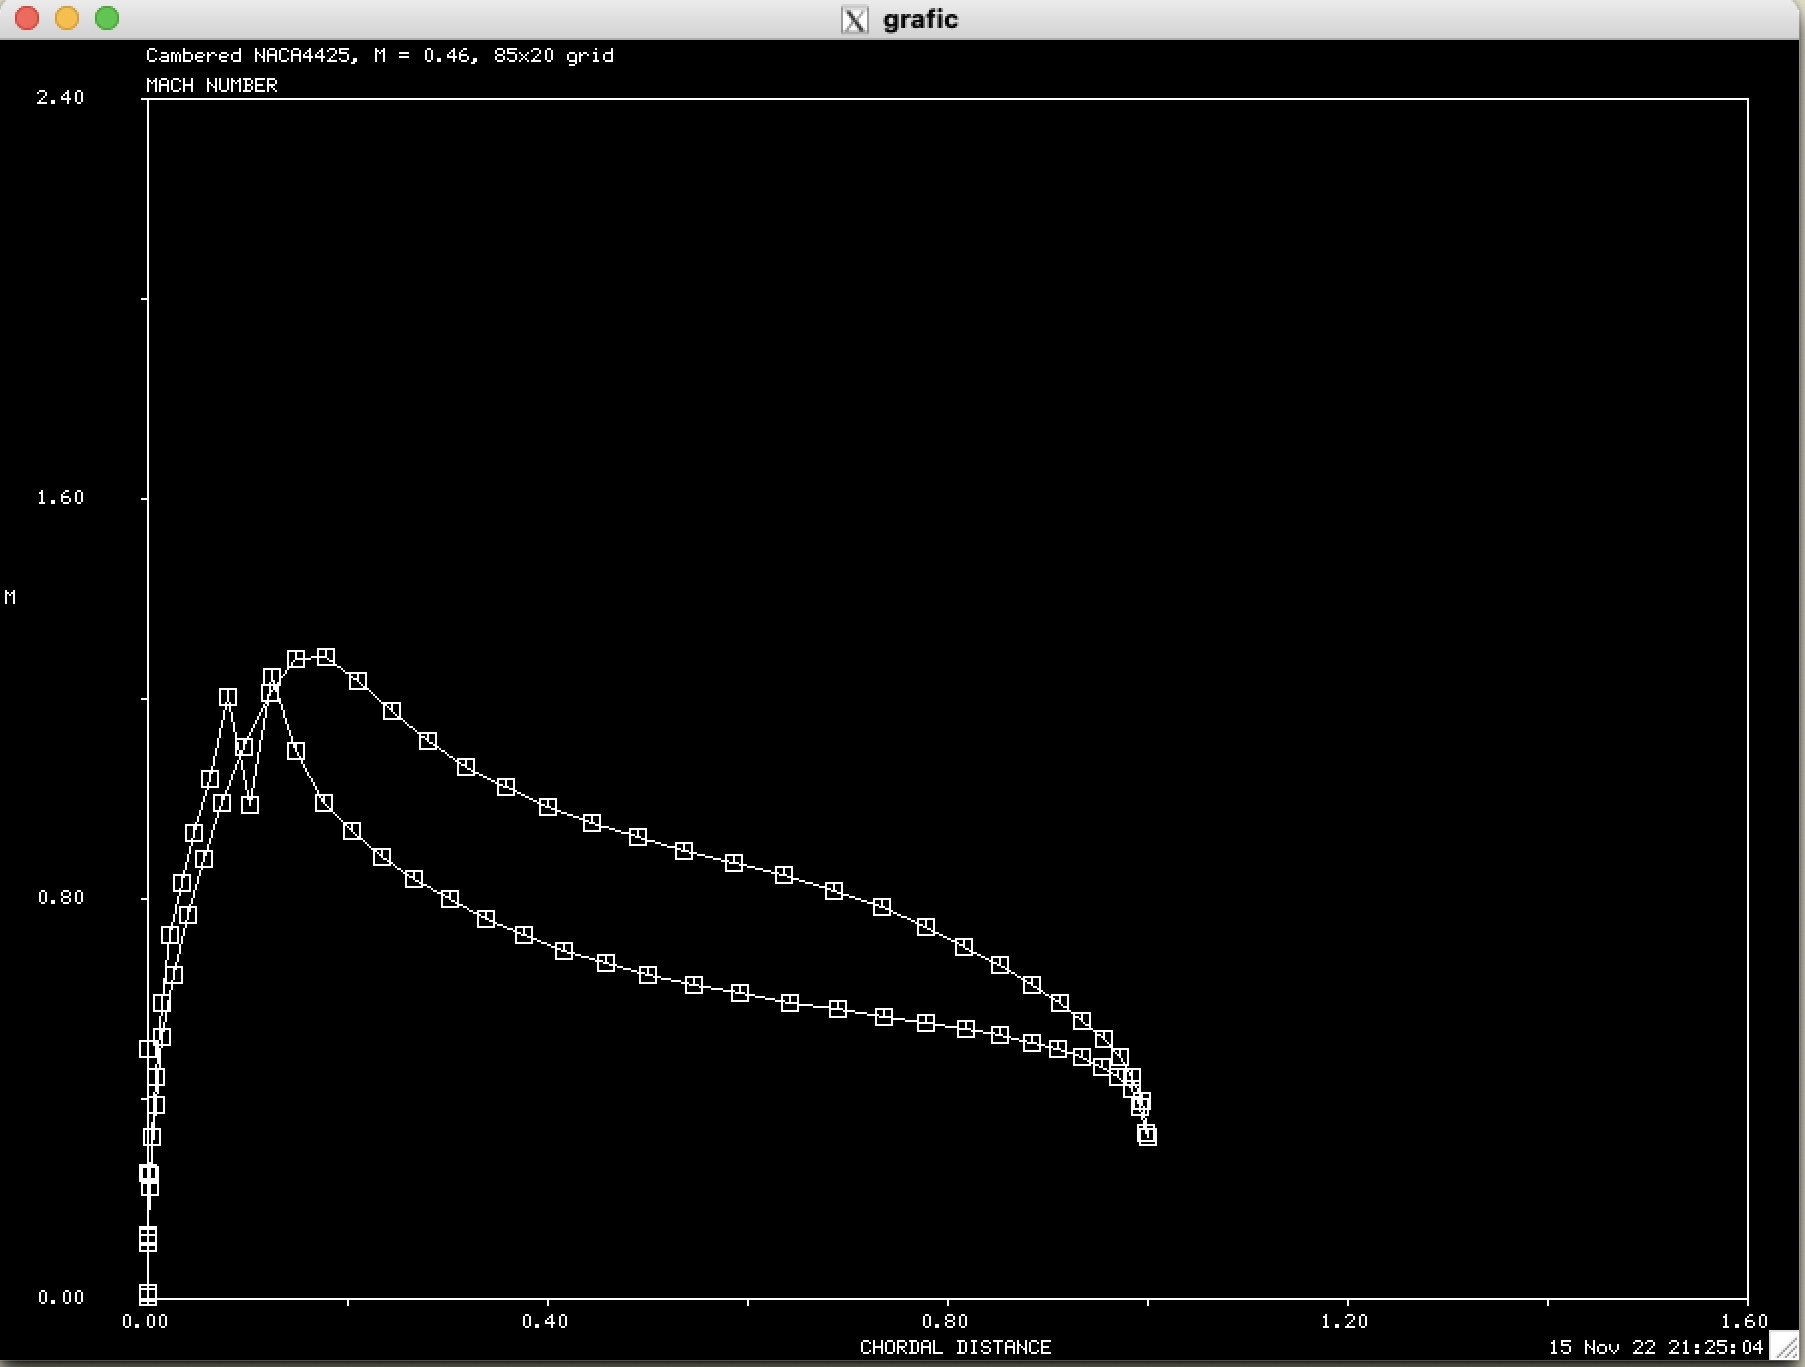
\includegraphics[width=1.0\textwidth]{/Mach.jpeg}
  \caption{Plot of the Surface Mach Number}
  \label{fig:Surf Mach}
\end{figure}

\end{document}